\chapter{Modelli di Regressione}
Un \textbf{Modello di regressione}, permette di poter valutare il valore di una variabile come funzione di ulteriori altre variabili. Per essere precisi, si definiscono:
\begin{itemize}
    \item \textbf{Response variables}: Le variabili che vengono stimate dal modello
    \item \textbf{Predictor variables}(o predictors o factors): Variabili utilizzare per andare a valutare le Response variables
\end{itemize}
I modelli regressivi possono essere di due principali tipologie:
\begin{itemize}
    \item \textbf{Lineare}: Modelli più utilizzati nella pratica. In generale vanno ad utilizzare tutti i parametri, ma molto spesso (ed anche in questo corso), si possono considerare dei modelli che si basano su un singolo predictor variable, tali modelli sono più semplici e vengono chiamati \textbf{simple linear regression models} 
    \item \textbf{Non Lineare}: Modelli non molto utilizzati che fanno uso delle relazioni non lineari tra le predictor variables
\end{itemize}

Oltre ad andare a definire i modelli e la loro struttura, bisogna definire quanto un modello sia qualitativamente buono rispetto ai dati utilizzati, quindi bisogna definire delle metriche di \textbf{qualità del modello}. Tali tecniche permettono di capire se il modello trovato è affine ai dati utilizzati per calcolarlo. Più precisamente, possiamo avere due tipologie di approcci al seguente problema:
\begin{itemize}
    \item \textbf{Approccio visuale}: Si va a valutare il modello in base a quanto questo sia "chiuso" rispetto ai valori considerati (quanto questo approssimi bene l'andamento delle mie osservazioni). Per comprendere bene tale concetto si può far riferimento alla figure [\ref{img:error-vision}]
    
    \item \textbf{Valutazione degli errori}: In primis devo capire come andare a definire il mio errore. Il modo più semplice per andarlo a definire è mediante la differenza tra il valore modellato su x (quindi la y calcolata) ed il valore reale rispetto alla variabile x. In genereale, l'errore, in questa modalità, viene definito come la distanza verticale tra il valore osservato e quello calcolato
\end{itemize}

\begin{figure}[h]
\centering
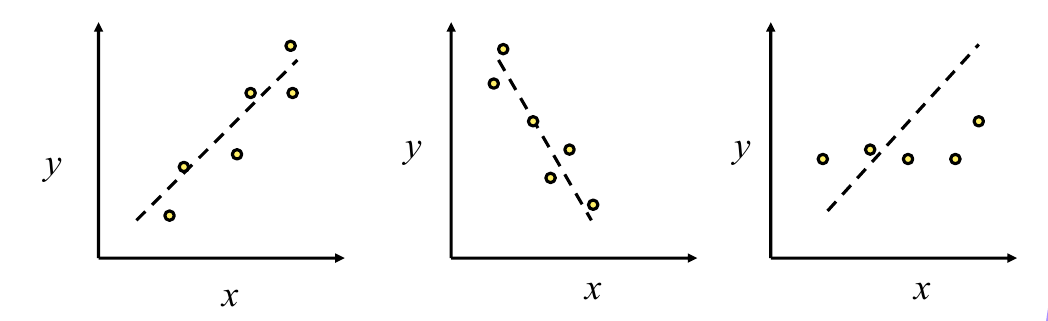
\includegraphics[width=.7\textwidth]{img/chapter-5/quality-regression.png}
\caption{Valutazione visiva dei modelli di regressione lineari}\label{img:error-vision}
\end{figure}

\section{Modelli di regressione lineari semplici}
I \textbf{simple linear regression model}(modelli di regressione lineare semplici), sono dei modelli che hanno un singolo parameter predictor. Queste presupposizione rende più semplice la trattazione di tali modelli, in particolare, il loro calcolo. Per comprendere meglio come si vanno a stimare i parametri del semplice modello lineare, bisogna passare per i \textbf{parametri di qualità del modello}. Più precisamente dalla valutazione dell'errore.  
Andando ad aggiungere più formalismo:\\
Considerando le \(n\) osservazioni: 
    \[(x_1, y_1), (x_2, y_2), \dots, (x_n, y_n)\]
    si va a costruire un modello lineare come: 
    \[\hat{y} = b_0 + b_1*x\]
    basato su tali osservazioni. Per valutare l'errore si prosegue nel calcolo del residuo come:
    \[e_i = y_i - \hat{y}_i\]
Con tale definizione, si può proseguire andando ad imporre la condizione, che la somma di tutti i residui sia pari a 0:
\[
\sum_{i=1}^{n}e_i = \sum_{i=1}^{n}(y_i - \hat{y}_i)=\sum_{i=1}^{n}(y_i - b_0 - b_1*x_i) =  0
\]
Andando a risolvere tale equazione non si troverebbe una \textbf{soluzione univoca}, poichè si avrebbe una equazione in 2 incognite, che quindi ha infinito alla 1 soluzioni. Pertanto vi è richiesto di definire un'ulteriore equazione, ovvero quella che fa riferimento all'\textbf{SSE}(Sum of Squared Error), che dev'essere minimizzato, ed è definito come:
\[
SSE = \sum_{i=1}^{n}e_i = \sum_{i=1}^{n}(y_i - b_0 - b_1*x_i)^2
\]
Questo però è un problema di minimizzazione vincolata, che quindi viene risolto in certi modi utilizzando varie tecniche. Noi utilizzeremo una tecnica pervenuta dall'esame di analisi 1, ovvero andremo a derivare la funzione quadrata e a porla uguale a 1. 

\begin{info}
\textit{Il prof non ha dato molto peso a questa parte, banalizzandola particolarmente. Di seguito, però, si riporta la dimostrazione per il calcolo dei coefficienti b1 e b0}
\\
Partendo dalla media dei residui e ponendola uguale a 0, si ottiene che:
\[
\frac{1}{n}\sum_{i=1}^{n}e_i = \frac{1}{n}\sum_{i=1}^{n}(y_i - b_0 - b_1 * x_i) = \overline{y} - b_0 - b_1 * \overline{x} = 0
\]
Da cui:
\[
b_0 = \overline{y} - b_1*\overline{x}
\]
Andando a sostituire tale definizione nella formula di calcolo dell'errore si avrebbe:
\[
e_i = y_i - \overline{y} + b_1*\overline{x} - b_1 * x_i = (y_i - \overline{y}) - b_1*(x_i - \overline{x})
\]
Qui mi fermo e vado a valutare l'errore quadratico, come:
\[
\frac{SSE}{n-1} = \frac{1}{n-1}\sum_{i=1}^{n}e_i^2 = \frac{1}{n-1}\sum_{i=1}^{n}\left ( (y_i - \overline{y}) - b_1*(x_i - \overline{x}) \right )^2=
\]
\[
= \frac{1}{n-1}\sum_{i=1}^{n}(y_i - \overline{y})^2 + \frac{b_1^2}{n-1}\sum_{i=1}^{n}(x_i - \overline{x})^2 - \frac{2\ b_1}{n-1}\sum_{i=1}^{n}((y_i - \overline{y})*(x_i - \overline{x}))
\]
Andando a denominare \(s_y = \sqrt{\frac{1}{n-1}\sum_{i=1}^{n}(y_i - \overline{y})^2}\), \(s_x = \sqrt{\frac{1}{n-1}\sum_{i=1}^{n}(x_i - \overline{x})^2}\) e \(s_{xy} = \sqrt{\frac{1}{n-1}\sum_{i=1}^{n}((y_i - \overline{y})*(x_i - \overline{x}))}\), si ottiene:
\[
\frac{SSE}{n-1} = s_y^2 + b_1^2 s_x^2 - 2 b_1 s_{xy}^2
\]
Andando a derivare rispetto a \(b_1\) si ottiene:
\[
\frac{1}{n-1}\frac{d SSE}{d b_1} = 2 b_1 s_x^2 - 2 s_{xy}^2 = 0
\]
da cui, si può calcolare \(b_1\) come:
\[
b_1 = \frac{s_{xy}^2}{s_{x}^2} = \frac{\sum_{i=1}^{n}((y_i - \overline{y})*(x_i - \overline{x}))}{\sum_{i=1}^{n}(x_i - \overline{x})^2}
\]
Affiancando a tale equazione quella calcolata in precedenza per \(b_0\), allora si ha la coppia di equazioni adatta per minimizzare l'SSE e valutare un modello di regressione quanto più possibile di qualità
\end{info}

In particolare, la valutazione che vado a fare del parametro \(b_1\) è legata fortemente al \textbf{trend} che i miei dati potrebbero avere. Quando \(b_1\) è un valore diverso da 0, allora ciò vuol dire che si è trovato un trend all'interno dei dati. Questo è causato dal fatto che la valutazione del valore \(b_1\) sia dipendente da un operazione di "correlazione" tra i valori predittori (predictor variables) ed i parametri di risposta (Response variables). 

\subsection{Devianze}
Come illustrato in precedenza, l'errore che viene commesso viene valutato come la somma dei quadrati delle deviazioni, il che quindi ci fa pensare alla definizione delle \textbf{devianze}. La devianza, in particolare, viene utilizzata all'interno della valutazione dell'errore, perchè rispetta la relazione triangolare, ovvero, la somma delle devianze ottenute da una separazione dei dati, è uguale alla devianza totale. Per applicare tale concetto al caso dei modelli lineari è utile andare a definire i seguenti concetti:
\begin{itemize}
    \item \textbf{SSE}(Sum of Squares for Errors): Si va ad effettuare la somma dei quadrati degli errori (deviazioni) commesse dal modello. Spesso può anche essere chiamato \textbf{Residual Sum of Squares}.
    \[
    SSE = \sum_{i=1}^{n}(y_i - \hat{y}_i)^2
    \]

    \item \textbf{SST}(Total Sum of Squares): Questa è la devianza associata alla variabile \(y\) e va a valutare tutta la sua variabilità.
    \[
    SST = \sum_{i=1}^{n}(y_i - \overline{y})^2
    \]

    \item \textbf{SSR}(Sum of Squares for regression): Devianza associata alla variabile \(\hat{y}\) e va a valutare la sua variabilità.
    \[
    SSR = \sum_{i=1}^{n}(\hat{y}_i - \overline{y})^2
    \]
\end{itemize}

Tali valori sono legati tra loro mediante la seguente relazione:
\[
SST = SSR + SSE
\]

che è dimostrabile sia algebricamente che matematicamente, ma ciò prescinde dagli obbiettivi del corso (in gnerale bisognerebbe andare au utilizzare un approccio algebrico matriciale non proprio semplice, ma come detto, tale dimostrazione prescinde dagli obbiettivi del corso).

\begin{info}
\textit{Tale dimostrazione prescinde dalle conoscenze del corso. Nonostante sia presente nel materiale fornito a lezione, tale dimostrazione non è richiesta ai fini dell'esame}

\textbf{Dimostrazione della relazione triangolare}
\\
Per capire come effettuare tale dimostrazione, si parte dal ridefinire il seguente problema:
\\
\textbf{Ipotesi}
\\
Si è utilizzato un modello di regressione lineare che calcola \(b_0\) e \(b_1\) partendo dalle seguenti presupposizioni:
\[
\overline{e} = \frac{1}{n}\sum_{i=1}^{n}e_i = 0
\]
\[
\frac{dSSE}{db_1} = 0 \implies \frac{d(\sum_{i=1}^{n}(y_i - b_0 - b_1x_i)^2)}{db_1} = -2\sum_{i=1}^{n}(e_i x_i) = 0
\]
\\
\textbf{Dimostrazione}
\\
A partire dalla definizione di SST, si effettuano i seguenti passaggi algebrici:
\[
SST = \sum_{i=1}^{n}(y_i - \overline{y})^2 = \sum_{i=1}^{n}[(y_i - \hat{y}_i) + (\hat{y_i} - \overline{y})]^2=
\]
\[
= \sum_{i=1}^{n}[(y_i - \hat{y}_i)^2 + (\hat{y}_i - \overline{y})^2 + 2 (y_i - \hat{y}_i) (\hat{y_i} - \overline{y})] = SSE + SSR + 2 \sum_{i=1}^{n}e_i(\hat{y}_i - \overline{y}) = 
\]
\[
= SSE + SSR + 2 (\sum_{i=1}^{n}e_i \hat{y}_i - \sum_{i=1}^{n}e_i \overline{y})
\]

Da questo risultato, date le ipotesi, si può dedurre che il secondo termine: \(\left [ \sum_{i=1}^{n}e_i \overline{y}\right ]\) è 0, dato che sarebbe il calcolo della somma degli errori per una costante (che annulla tale somma). Per quanto riguarda invece l'altro termine, questo va analizzato nel seguente modo:
\[
\sum_{i=1}^{n}e_i \hat{y}_i = \sum_{i=1}^{n}e_i (b_0 + b_1 x_i) = \sum_{i=1}^{n}b_0 e_i + \sum_{i=1}^{n}b_1 x_i e_i = 0
\]

Il primo termine di questa equazione, si annulla per lo stesso motivo del precedente, mentre il secondo termine si annulla per via che \(b_1\) è una costante e che il termine \(\sum_{i=1}^{n}e_i x_i\), date le ipotesi, è nullo.

Pertanto, considerate tali "annullamenti" si ricava la tesi, ovvero la relazione triangolare:
\[
SST = SSE + SSR
\]
\end{info}

\subsubsection{Coefficiente di determinazione}
Per valutare la qualità di un modello lineare, si possono utilizzare i tre parametri precedentemente presentati, ovvero: \(SSE, SSR\) ed \(SST\). Da tali valori possiamo calcolare il \textbf{coefficiente di determinazione}, che ci dice la percentuale rispetto alla devianza totale, della devianza presa dall'algoritmo di regressione (la devianza della regressione se è maggiore di quella dell'errore è buon segno, dato che si ha una buona rappresentabilità dei dati che si ha in ingresso). Per il calcolo di tale coefficente, quindi, si effettua il seguente rapporto:
\[
R^2 = \frac{SSR}{SST} = \frac{SST-SSE}{SST}
\]

Più \(R^2\) è alto e più il modello lineare è di qualità. Vi è però un problema, \(R^2\) cresce al crescere degli elementi considerati, il che potrebbe sembrare un bene, ma non è così, dato che non è la cardinalità della popolazione che mi dice che c'è un trend trai i dati. Pertanto, si è definita una versione normalizzata della \(R^2\), detta \textbf{adjusted \(\mathbf{R^2}\)}.

\subsubsection{Adjusted \(\mathbf{R^2}\)}
L'\textbf{Adjusted \(\mathbf{R^2}\)} va a valutare la percentuale di devianza che è stata coperta, essa, però, tiene conto anche del numero di parametri indipendenti all'interno del mio dataset. Più parametri dipendenti ho e maggiore potrebbe essere la varianza catturata dal trend. Quindi, considerando \(k\) il numero di elementi indipendenti del mio dataset ed \(n\) il numero totale di elementi. Sì definisce adjusted \(R^2\) come:
\[
\overline{R}^2 = 1 - \frac{(1 - R^2)(n-1)}{n-k-1}
\]

Dove non tengo solo conto della quantità di dati, ma anche della loro indipendenza. Più i dati sono dipendenti e più il trend che si va a trovare è conforme ai dati da rappresentare, mentre, più questi sono indipendenti, e più risulta difficile andarli a valutare. Ciò, quindi va ad aggiungere un "peso specifico" alla variabile aggiunta rispetto alle altre.

\subsubsection{Deviazione standard degli errori}
Una volta ottenuta la somma di tutti gli errori, ci è richiesto di andare a calcolare anche il possibile intervallo di confidenza associato a tali valori. Per farlo, in primis, bisogna definire come calcolare la deviazione standard. Per farlo si prosegue con la seguente formula:
\[
s_e = \sqrt{\frac{SSE}{n-2}}
\] 
Si divide l'SSE per \(n-2\) poichè questi sono i gradi di libertà associati all'SSE. Ciò è dovuto principalmente al fatto che si sono utilizzati 2 gradi di libertà per determinare i valori di \(b_0\) e \(b_1\). 
Oltretutto, si può definire anche l'\textbf{MSE}(Mean Squared Error) come: \(MSE = \frac{SSE}{n-2}\).

Una cosa curiosa da notare è come possiamo andare a valutare i gradi di libertà sommando i vari gradi di libertà associati ad ogni varianza. \(n-1 = (n-1) + 1\) che sarebbero i gradi di libertà di \(SST = SSE + SSR\)


\subsection{Parameters and Statistics}
Fino ad ora abbiamo ragionato con le statistiche \(b_0\) e \(b_1\) (quindi questi valori fanno riferimenti ai risultati ottenuti su un singolo campione di osservazioni). In generale il modello associato alla popolazione, quindi la valutazione dei parametri, viene effettuata in altri modi. I parametri associati alla popolazione, in particolare, vengono denotati come:
\[
y = \beta_0 + \beta_1 x
\]
dati tali valori, ho bisogno di trovare un modo per correlare le statistiche con i parametri del mio problema. Pertanto, come per altri problemi di statistica inferenziale, quello che si va a fare è sostenzialmente, valutare un intervallo di confidenza con un certo livello di confidenza, e sulla base di tali intervalli, trovare un possibile valore per i parametri associati alla popolazione.

Gli intervalli di confidenza vengono gestiti mediante una t-student, dato che non si conosce la "varianza" dei dati originali (Non ho ancora trovato il modello originale). Pertanto, vado a calcolarmi le devizioni standard associate al parametro \(b_0\) e \(b_1\) come:
\[
s_{b_0} = s_e \left [ \frac{1}{n} + \frac{\overline{x}^2}{\sum_{i=1}^{n}x_i^2 - n \overline{x}^2}\right ]^{1/2}
\]
\[
s_{b_1} = \frac{s_e}{[\sum_{i=1}^{n}x_i^2 - n \overline{x}^2]^{1/2}}
\]
Da cui, prefissando un livello di confidenza pari a \(100*(1-\alpha)\%\), posso ricavare l'intervallo di confidenza per entrambi i parametri. Per farlo vado a considerare in primis il valore della t-student per \(1 - \alpha/2\) con \(n - 2\) gradi di libertà. (\(t_{1-\alpha/2; n-2}\)). Da cui ricavo gli intervalli di confidenza come:
\[
b_0 \mp t s_{b_0}
\]
\[
b_1 \mp t s_{b_1}
\]
Bisogna fare attenzione a tali intervalli, sopratutto per il parametro \(b_1\), poichè, se l'intervallo di confidenza contiene 0, nulla lo esclude come valore, il che potrebbe pregiudicare la mancanza di un trend tra i dati.

\begin{info}
\textit{Questa parte il prof in aula l'ha skippata. Viene aggiunta solo a scopo di completezza e conoscenza}
\\
Precedentemente si è valutato l'intervallo di confidenza dei parametri. Ma si potrebbe andare a valutare anche l'intervallo di confidenza della media dei valori che possono essere assunti da un algoritmo di regressione. Pertanto. Sì definisce \(m\) il numero di osservazioni totali nella popolazione, \(n\) il numero di osservazioni del singolo campione, definito tutto ciò, si definisce la deviazione standard associata alla media dei valori \(y\) come:
\[
s_{\hat{y}_{mp} = s_e \left [ \frac{1}{m} + \frac{1}{n} + \frac{(x_p - \overline{x})^2}{\sum_{i=1}^{n}x_i^2 - n \overline{x}^2}\right ]^{1/2}}
\]
\end{info}

\subsection{Visual Tests for Assumptions}
Andare ad effettuare la regressione richiede  he siano verificate una serie di assunzioni rispetto alle variabili che si stanno andando a considerare.
In generale le assunzioni che si vanno ad effettuare sono:
\begin{itemize}
    \item \textbf{Relazione lineare}: La relazione tra la variabile \(y\) e la variabile \(x\) è lineare
    \item \textbf{Predictor non stocastico}: La variabile \(x\) dev'essere non-stocastica (il che vuol dire che non ha un comportamento casuale) e non deve avere alcun tipo di errore di misurazione
    \item \textbf{Indipendenza degli Errori}: Il modello degli errori dev'essere indipendente
    \item \textbf{Omoschedasticità degli errori}(Homoschedasticity of errors): Gli errori devono essere normalmente distribuiti, la cui media è nulla e la deviazione standard costante.
\end{itemize}

\begin{info}
\textit{Tale pezzo è stato inserito solo a scopo informativo, ma non viene richiesto ai fini dello svolgimento dell'esame}
\\
\textbf{Omoschedasticità}
\\
La omoschedasticità si verifica quando la varianza del termine d’errore \(\epsilon_i\)
è costante per tutte le osservazioni, cioè:
\[
Var(\epsilon_i) = \sigma
\]
In termini intuitivi, significa che la dispersione dei punti osservati attorno alla retta di regressione è uniforme: gli errori non diventano né più grandi né più piccoli al crescere (o al variare) di \(x_i\).
Se invece la varianza degli errori cresce (o decresce) con \(x_i\), si ha \textbf{eteroschedasticità}, indice di una modellazione dei parametri non adeguata o di un modello che non cattura correttamente la relazione tra le variabili.
\end{info}

Definite le assunzioni che bisogna fare rispetto ai dati, è utile, andarsi a plottare i valori che si voglione mettere in relazione (\(x\) ed \(y\)), per valutare se effettuare una regressione lineare o meno.
Per effettuare tali test visuali vi sono tecniche per ogni tipologia di assunzione che si vuole verificare.

\newpage
\subsubsection{Relazione Lineare}
In prima battuta mi conviene andare a plottare i dati di cui voglio valutare un'algoritmo di regressione, in modo da capire se tra essi sussiste una relazione d'ordine o meno. Per degli esempi fare riferimento alla figura [\ref{img:regression-relations}]

\begin{figure}[h]
\centering
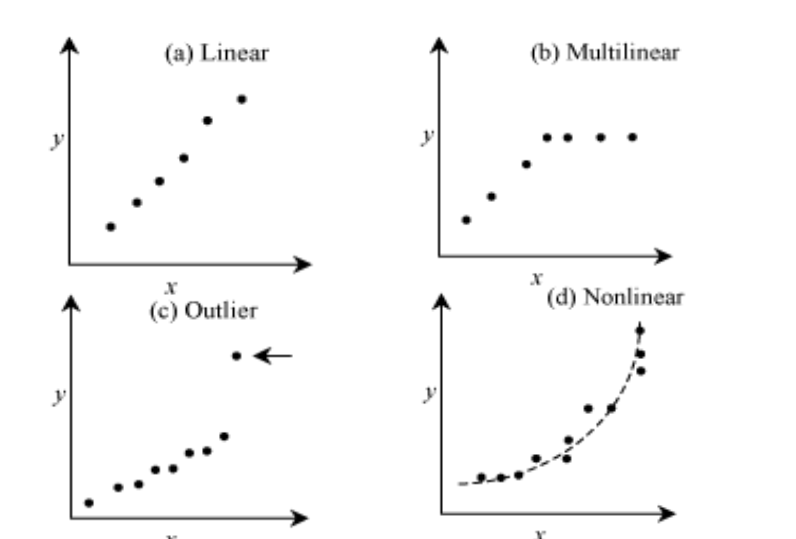
\includegraphics[width=.7\textwidth]{img/chapter-5/regression-relations.png}
\caption{Esempi di dati in relazione tra loro}\label{img:regression-relations}
\end{figure}

\subsubsection{Indipendenza degli errori}
Per verificare l'indipendenza degli errori a livello grafico, si va a plottare la distribuzione degli errori \(e_i\) rispetto alle corrispettive variabili predette \(\hat{y}_i\), ciò viene fatto per verificare se ci sia dipendenza in base alla variabile predetta, e quindi "scagionare" dei trend indesiderati all'interno degli errori. Per comprendere tale concetto, visualizzare l'immagine [\ref{img:independent-errors}], che mostra degli esempi di errori sia indipendenti, che dipendenti in diverse forme.

\begin{figure}[h]
\centering
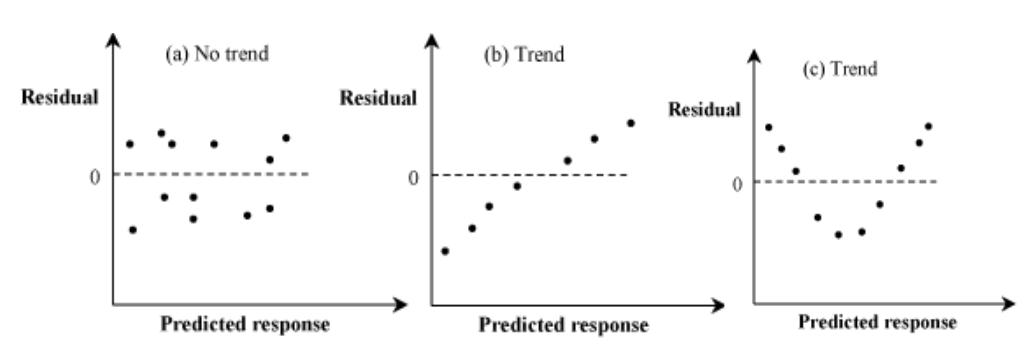
\includegraphics[width=.8\textwidth]{img/chapter-5/independet-errors.png}
\caption{Esempi di distribuzioni degli errori rispetto alla variabile \(\hat{y}_i\)}\label{img:independent-errors}
\end{figure}

A volte, è conveniente andare a plottare gli errori \(e_i\) in riferimento al numero dell'esperimento stesso \(i\), in modo da verificare se magari ci sono effetti nascosti (errata inizializzazione, procedure sperimentali) o delle condizioni dell'ambiente (temperatura ed umidità) che vanno ad incidere su tali errori (per fare ciò vado sempre a verificare i possibili trend presenti all'interno di tale relazione). Esempi di tali plot sono quelli presenti in figura [\ref{img:errors-side-effect}]

\begin{figure}[h]
\centering
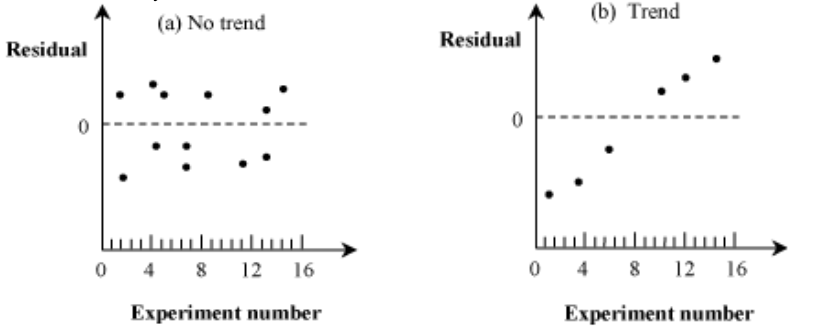
\includegraphics[width=.7\textwidth]{img/chapter-5/errors-side-effect.png}
\caption{Plotting degli errori rispetto alla posizione di valutazione}\label{img:errors-side-effect}
\end{figure}

\subsubsection{Errori distribuiti normalmente}
Per verificare se gli errori seguono una distribuzione normale, ci viene in aiuto il \textbf{Quantile-Quantile plotting}, che mette in relazione la distribuzione ottenuta dagli errori, rispetto ad una distribuzione normale. Esempi di applicazione della QQ-Plot sono rappresentati in figura [\ref{img:qqplot-errors}]

\begin{figure}[h]
\centering
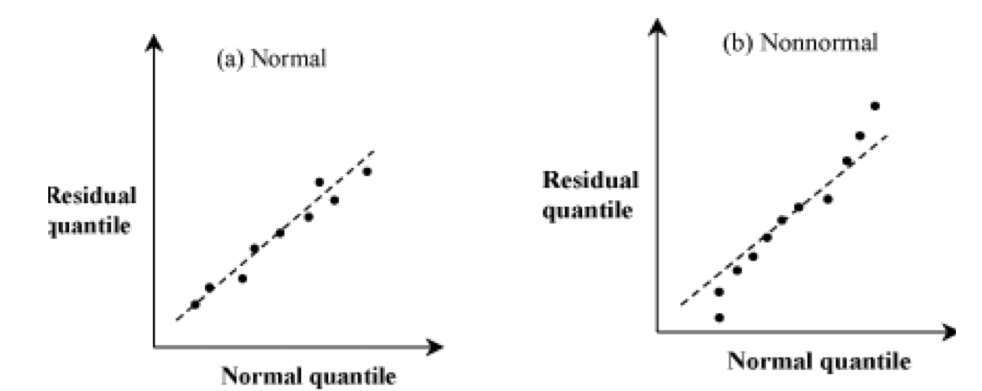
\includegraphics[width=.7\textwidth]{img/chapter-5/qqplot-errors.png}
\caption{QQ-Plot per le distribuzioni degli errori}\label{img:qqplot-errors}
\end{figure}

\subsubsection{Deviazione standard costante}
Quello che si va a fare, si va a plottare gli errori in riferimento alla risposta predetta (che dipende dalle predictor variables), andando a valutare se ci sono relazioni. Tale test visivo ci permette di verificare l'\textbf{Omoschedasticità}(Deviazione standard costante e media nulla) [Questa è la definizione mostrata a lezione e dalle dispense, anche se sui testi e in rete la definizione comprende solo la parte di deviazione standard (solo ipotesi di costanza di tale valore)]. Guardando il grafico, è importante stare attenti ad osservare se c'è un trend degli errori rispetto alla risposta predetta. Poichè in tal caso, non si possono fare ipotesi sulla costanza della varianza. Esempi di tali grafici sono quelli mostrati alla figure [\ref{img:constant-deviation}]

\begin{figure}[h]
\centering
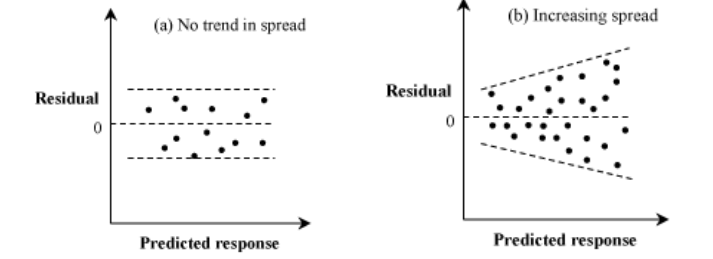
\includegraphics[width=.7\textwidth]{img/chapter-5/constant-deviation.png}
\caption{Distribuzione degli errori}\label{img:constant-deviation}
\end{figure}


L'Omoschedasticità si può verificare (o confermare) anche mediante l'utilizzo di uno specifico test statistico. Vi sono varie tecniche e modelli con cui tale test può essere effettuato, tali tecniche vanno sotto il nome di ANOVA (Analysis Of Variance) in letteratura. Ad esempio: 
\begin{itemize}

  \item \textbf{p-value:} 
  È la probabilità di osservare un risultato uguale o più estremo di quello ottenuto, assumendo vera l’ipotesi nulla. 
  Nei test di uguaglianza delle varianze indica quanto è plausibile che le varianze siano effettivamente uguali. 
  Se $p < \alpha$ (es. 0.05), si rifiuta l’ipotesi nulla: le varianze non sono uguali.

  \item \textbf{Test di Levene:} 
  Verifica se le varianze di più campioni sono uguali, basandosi sulle deviazioni assolute dalla media (o mediana) di ciascun campione. 
  È più robusto del test di Bartlett rispetto alla non-normalità. 
  Ipotesi nulla: le varianze dei campioni sono uguali.

  \item \textbf{Test di Brown–Forsythe:} 
  Variante del test di Levene che utilizza la mediana invece della media, rendendolo ancora più robusto a outlier e distribuzioni asimmetriche. 
  Ipotesi nulla: le varianze dei campioni sono uguali. 
  È consigliato quando la normalità non può essere assunta.

  \item \textbf{Test di Bartlett:} 
  Test classico per verificare l’uguaglianza delle varianze basato su una statistica $\chi^2$. 
  È potente se i dati sono normali, ma molto sensibile alle deviazioni dalla normalità. 
  Ipotesi nulla: tutte le varianze sono uguali; se $p < \alpha$, si conclude che almeno una varianza differisce.
    
  \item Ce ne sono altri ma prescindono da tale corso

\end{itemize}

Nel caso in cui, invece, i dati siano normali ma Eteroschedatici, allora è conveniente utilizzare il \textbf{Welch's t-test}. 

\begin{warn}
Le specifiche fatte sulle varie tecniche sopraelencate sono state aggiunte per un leggero grado di comprensione in più. Ma non sono richieste al fine di effettuare l'esame
\end{warn}

\subsection{Regressione Lineare Non parametrica}
Quando si parla di \textbf{Regressione lineare non parametrica}, si intende quell'insieme di tecniche che cerca un trend di un certo tipo, senza fare alcuna ipotesi sulla forma della popolazione o sulla distribuzione che i dati devono avere, richiede solo che ci sia indipendenza sui dati presenti. 
Per tali tipologie di test si utilizza il \textbf{test di Mann-Kendal}, che va a valutare la tendenza di una serie, e verifica se questa sia monotona o meno. Formalizzando tale concetto, andiamo a definirne le specifiche:
\\
Dato un insieme di una coppia di valori, di cui si vuole verificare un eventuale trend (insieme di punti nel piano), \(x_1, x_2, \dots, x_n\) e \(y_1, y_2, \dots, y_n\), si definisce un valore \(S\) che sarà utilizzato per la verifica. Sì definisce il valore \(S\) come:
\[
S = \sum_{i < j}sign((x_j - x_i)(y_j-y_i))
\]
Quindi si va ad effettuare una somma della valutazione dei parametri (se concordi si somma, se discordi si sottrae).
Più precisamente si va a controllare se i punti siano \textbf{concordanti} (Concordant, danno un contributo positivo) o \textbf{discordanti} (discordant, danno un contributo negativo). Per comprendere tale relazione guardare l'immagine [\ref{img:concordant-discordant}].

\begin{figure}[h]
\centering
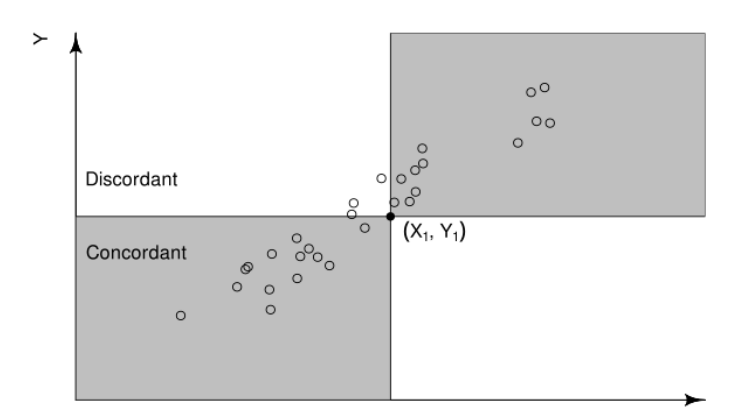
\includegraphics[width=.7\textwidth]{img/chapter-5/concordant-discordant.png}
\caption{Punti concordanti e discordanti}\label{img:concordant-discordant}
\end{figure}

Il valore di \(S\) ci permette di capire, in base al segno ed al valore che assume, se i dati hanno una certa tendenza. Per capire al meglio tale tendenza, ci calcola un'altro parametro \(\tau_a\) che indica il \textbf{coefficente di correlazione}. Più \(S\) e \(\tau_a\) sono grandi e più con forza posso rigettare l'ipotesi nulla (quella associata alla mancanza di trend nei dati). 
Per calcolare la \(\tau_a\) si effettua il seguente calcolo
\[
\tau_a = \frac{S}{\binom{n}{2}} = \frac{S}{\frac{n(n-1)}{2}}
\]
Con tale valore, vado a riscalare il valore di \(S\) ad un range \(-1 \leq \tau_a \leq 1\), poichè è come se stessi andando ad aggiungere un peso per ogni valore "valutato".

Dato che solitamente, si potrebbe incappare nel problema dei "pareggi" (ovvero valori nulli). Si può andare a valutare un'altro parametro che è:
\[
\tau_b = \frac{S}{\sqrt{(\binom{n}{2} - n_1)(\binom{n}{2}-n_2)}}
\]
Dove \(n_1\) ed \(n_2\) sono il numero di pareggi per ogni campione che si va a considerare (\(x_i\) ed \(y_i\)).

\subsubsection{Procedura di Sen}
Un modo per essere più robusti agli outlier e trovare un eventuale trend, è la seguente procedura. Considerato che i dati mostrati \textbf{posseggono tra loro un trend}, si vanno a valutare le pendenze, e si seleziona il valore della mediana tra queste.
Per la valutazione delle pendenze si prosegue nel seguente calcolo:
\[
slope_{ij} = \frac{y_j - y_i}{x_j - x_i}
\]

\section{Altri modelli di regressione}
A volte la \textbf{Simple linear regression} non riesce a compensare tutti i casi richiesti o leggermente più complessi. Pertanto è utile andare ad esplorare diverse tecniche che ne permettono una buona stima

\subsection{Regressione Lineare Multipla}
A differenza della regressione lineare semplice, dove si cerca una relazione tra una singola variabile predictor e una singola predictable variable. Talvolta, utilizzare tale metodologia può essere limitante. Pertanto si definisce la \textbf{Multiple Linear Regression}(Regressione Lineare Multipla), che va a considerare una relazione \textbf{lineare} tra diverse variabili predictor. Per ogni campione si effettua una predizione rispetto al numero di parametri che si sono andari a utilizzare (predictor variables). Formalmente, definendo:
\begin{itemize}
    \item \(\mathbf{x_{ij}}\): Valore dell'attributo j-esimo per il campione i-esimo
    \item \(\mathbf{y_j}\): j-esimo valore predetto
    \item \(\mathbf{b_i}\): coefficente associato al parametro i-esimo
    \item \(\mathbf{e_j}\): Errore associato al j-esimo valore predetto
\end{itemize}

si può scrivere la relazione tra i predictor variables e le predictable variables come:
\[
y_j = b_0 + b_1 x_{j1} + b_2 x_{j2} + \dots + b_k x_{jk} + e_j
\]
Oppure in maniera estesa come:
\[
\begin{bmatrix}
y_1 \\
y_2 \\
\dots\\
y_n
\end{bmatrix}
= 
\begin{bmatrix}
1 & x_{11} & x_{12} & \dots & x_{1k}\\
1 & x_{21} & x_{22} & \dots & x_{2k}\\
\dots & \dots & \dots & \dots & \dots \\
1 & x_{n1} & x_{n2} & \dots & x_{nk}
\end{bmatrix}
\begin{bmatrix}
b_0 \\
b_1 \\
\dots \\
b_n
\end{bmatrix}
+
\begin{bmatrix}
e_1\\
e_2\\
\dots\\
e_n
\end{bmatrix}
\]
Con la notazione vettoriale
\[
\mathbf{\underline{y}} = \underline{\underline{\mathbf{X}}}\ \underline{\mathbf{b}}+\underline{\mathbf{e}}
\]

Per il calcolo dei parametri, si cerca di andare a minimizzare la formula dell'errore, ovvero:
\[
e_i = y_i - b_0 - b_1 x_{i1} - b_2 x_{i2} - \dots - b_k x_{ik} 
\]
\[
\sum_{i=1}^{n}e_i^2 = \sum_{i=1}^{n}(y_i - b_0 - b_1 x_{i1} - b_2 x_{i2} - \dots - b_k x_{ik})^2
\]

Scrivendo \(\sum_{i=1}^{n}e_i^2 = (\underline{y}-\underline{\underline{X}}\ \underline{b})^T(\underline{y}-\underline{\underline{X}} \ \underline{b})\), da cui, derivando rispetto a \(b\), si ottiene:
\[
\underline{b} = (\underline{\underline{X}}^t\ \underline{\underline{X}})^{-1}\underline{\underline{X}}^T\ \underline{y}
\]

Compreso come effettuare la stima dei valori per effettuare la regressione lineare multipla, si prosegue nell'effettuazione della valutazione degli "errori", delle veriazioni e delle devianze.
Precisamente, partendo dalle variazione e dalle devianze, si ha che:
\[
SSY = \sum_{i=1}^{n}y_i^2, SS0= n\overline{y}^2
\]
\[
SST = SSY - SS0
\]
\[
SSR = SST - SSE
\]

Dove i gradi di libertà della SST sono sempre \(n-1\) mentre quelli della SSE sono \(n-k-1\). Si valutano, anche, il coefficiente di determinazione e la deviazione standard, come:
\[
R^2 = \frac{SSR}{SST}
\]
\[
s_e = \sqrt{\frac{SSE}{n-k-1}}
\]

Per il calcolo del \textbf{MSE}(Mean squared error), si effettua la seguente formula:
\[
MSE = \frac{SSE}{n-k-1}
\]

Mentre la deviazione standard dei parametri, viene valutata come:
\[
s_{b_j} = s_e\sqrt{c_{jj}} 
\]

dove \(c_{jj}\) è il j-esimo elemento diagonale della matrice \(\underline{\underline{C}} = (\underline{\underline{X}}^T\underline{\underline{X}})^{-1}\)

\subsection{Multicolinearità}
La \textbf{Multicolinearità} vuol dire effettuare la regressione con una dipendenza lineare tra le variabili predictor (tale situazione è detta colineare). Tale situazione, ci permette di capire che si avrebbe una variabile in più su cui si sta effettuando la regressione (quindi di per se, inutile). Quindi, solitamente, è utile capire se due variabili sono colineari o meno (correlate o meno). Per effettuare tale valutazione si va a calcolare la correlazione tra i due elementi, che poi viene valutata.
La correlazione tra i due elementi viene calcolata come:
\[
Correlation(x_1,x_2) = R_{x_1x_2} = 
\]
\[
=\frac{\sum_{i=1}^{n}x_{1i}x_{2i} - \frac{1}{n}\left(\sum_{i=1}^{n}x_{1i}\right)\left(\sum_{i=1}^{n}x_{2i}\right)}{\left[\sum_{i=1}^{n}x_{1i}^2 - \frac{1}{n}\left(\sum_{i=1}^{n}x_{1i}\right)\left(\sum_{i=1}^{n}x_{1i}\right) \right]^{1/2}\left[\sum_{i=1}^{n}x_{2i}^2 - \frac{1}{n}\left(\sum_{i=1}^{n}x_{2i}\right)\left(\sum_{i=1}^{n}x_{2i}\right) \right]^{1/2}}
\]

Quindi, aggiungere una variabile predictor non è detto che sia sempre una buona idea, poichè, la correlazione tra due predittori, riduce l'accuracy e va ad amplificare la varianza (Valori della matrice di correlazione vista in precedenza). 

\subsection{Regressione Curvilinea}
Talvolta, può capitare che la relazione presente tra \(y\) e \(x\) non sia lineare, ma che comunque racchiude una funzione non lineare. Quello che sostanzialmente si può andare a fare, è cercare una relazione lineare rispetto a funzioni non lineari. Per capire, immaginiamo che \(y\) ed \(x\) siano legate dalla legge \(y = bx^\alpha\), allore quello che si potrebbe andare a fare, è valutare il modello logaritmico di tale funzione come:
\[
ln(y) = ln(b)+ \alpha ln(x)
\]

Il che quindi mi consente di utilizzare le tecniche affrontate per la regressione lineare, per trovare i valori di \(b\) e \(\alpha\). Oltre a tale legame ce ne sono altri, che sono mostrati nella figura [\ref{img:trasformazioni-curvilinee}]

\begin{figure}[h]
\centering
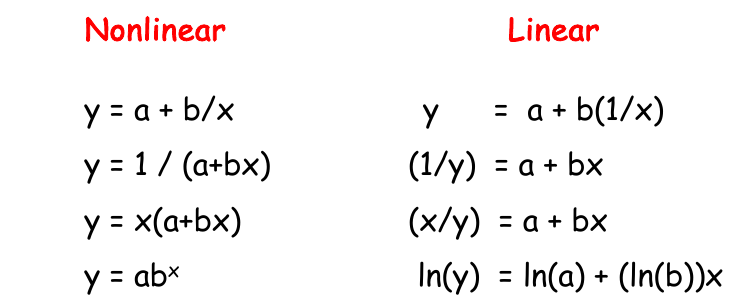
\includegraphics[width=.7\textwidth]{img/chapter-5/relazioni-curvilinee.png}
\caption{Forme di trasformazione di funzioni non lineari in relazioni lineari}\label{img:trasformazioni-curvilinee}
\end{figure}

\subsection{Outliers}
